\documentclass[12pt]{article}

% packages
\usepackage{a4wide}
\usepackage[english]{babel}
\usepackage{csquotes}
\usepackage{hyperref}
\usepackage{graphicx}
\usepackage{tocloft}
\usepackage{xcolor}
\usepackage{biblatex}
\addbibresource{../../biblio.bib}

% formatting
\renewcommand{\cftsecleader}{\cftdotfill{\cftdotsep}}   % points in table of contents
\setlength{\parskip}{\baselineskip}                     % add space between paragraphs


% attributes
\title{\underline{\textbf{ExaMA WP3 -- Dashboard Performances}}}
\author{Tanguy Pierre\\
            [1cm]
            Supervisors: V. Chabannes, J. Cladellas\\
            [2cm]
            University of Strasbourg}

\date{23rd of April}



% **********************  START  **********************
\begin{document}
    \maketitle      % titlepage to be improved


\newpage
\section{Introduction}

This work is part of the \textit{ExaMA} project, whose main objective is to design algorithms and methods
that will adapt in the best way to exascale machines and their imminent appearance.

Benchmarking is an unavoidable step for \textit{ExaMA}, as it needs to analyse and compare performances on systems
with different structures. These analyses will not only guide the developer team to improve the scalability of the different available tools,
but also ensure complete transparency during the evaluation process.

As launching tests on supercomputers isn't always easy because of their availability and costs, there is a real need to store the results.
In addition to this fact, it serves as a manner to verify that new features haven't caused any pullback in performance.
It is also important for this project to create a well-structured database for analyses depending on specific context, like machine or application.

It is exactly what the \textit{Dashboard Performances} project is about: providing a clear and easy to use interface between tests and results.
This interface is already available at \url{https://feelpp.github.io/benchmarking/benchmarking/index.html}.


\section{Tools description}

For testing the implemented algorithms and trying to predict how they will behave, we will use \textit{ReFrame HPC}\cite*{ReFrame}.
ReFrame is a robust framework that allows to focus only on the algorithm by isolating the running code from the system's complexity.
It distinguishes between "performance by simulation step" and "performance by number of task", which are two unavoidable criteria when talking about HPC.
But for us, the most interesting feature is its ability to simulate exascale performance with regressions tests.

The algorithms we want to test will be from the \textit{Feel++}\cite*{Feelpp} library.
This is a "Finite Element Embedded Library in C++". It is used for solving physical problems, up to dimension 3,
through the resolution op partial differential equations employing continuous or discontinuous Galerkin methods.
\newpage
For reporting the results, we will use \textit{Antora}\cite*{Antora}. Antora gives the opportunity to publish documentation on the web.
The documentation needs to be written in \textit{AsciiDoc}. Once it's done, \textit{AsciiDoctor} will handle the conversion to \textit{html}
for responsiveness and browser compatibility.
\textit{AsciiDoc} offers the possibility to call python function directly within its file. With this approach, we will be able to provide dynamic content,
like graphs for example, for the documentation.

The \textit{Plotly}\cite*{Plotly} library will be used for data visualization. This graphing library offers various methods for displaying data.
what's particularly notable for our purposes is its interactivity. Together with its versatility, it perfectly fits the project's needs
regarding dynamism.


\section{Process}
Resources for publishing new documentation are already available in this repository. We need to adapt them to our new testsuite.\\
However, achieving this requires to integrate the previously mentioned tools in the following process:

\begin{figure}[h]
    \centering
    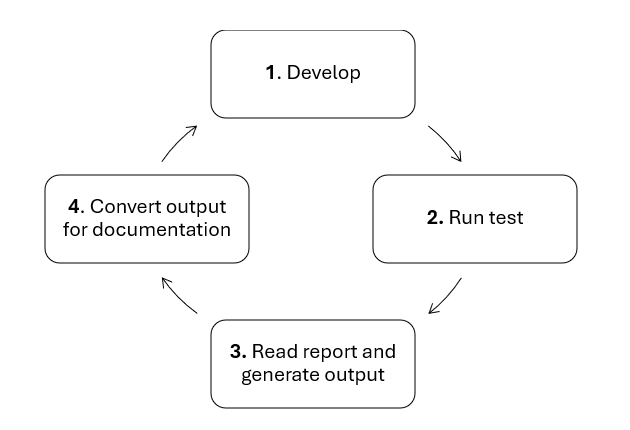
\includegraphics[width=0.8\textwidth]{../../illustrations/process.png}
\end{figure}

\newpage
\begin{enumerate}
    \item The first step of this cycle is of course to develop. This is the only manner to look forward regarding performances.
    Pushing or merging new test reports should also launch a new process.
    \item The workflow should automatically launch the specified tests using Reframe. The results will be transmitted in a .json file.
    If a code doesn't pass all the tests, a warning will appear in order to inform the dev team they have performance decline regarding the new code. In this case, the process will automatically stop.
    \item At first, we will extract the relative run reports data with a Python script. Then, the Python library \textit{Jinja2}\cite*{Jinja2} will generate an .adoc file containing plotting methods.
    \item The last step to convert the created .adoc file into .html for generating the website. As I mentioned before, this job is done by Antora together with AsciiDoctor.
\end{enumerate}

It's apparent that this task involves significant repetition. Therefore, we want our process to work on the most autonomous way possible. This leads us immediately to our main objective.



\section{Objectives}
\begin{itemize}
    \item Establish a \textbf{Continuous Integration/Continuous Deployment} workflow.
    This means that every time a new test is done and integrated into the repository main branch, a task will automatically be launched for updating the documentation site.
    \item Improve the \textbf{dashboard presentation}. We need to enhance the data visualization and add explanations to it for a better comprehension of the given results.
    \item Finding the appropriate values to analyse performances on a specific context can be difficult. Therefore, \textbf{representative tests} are essential for obtaining reliable results about the system behaviour.
    \item Provide a \textbf{database} for easy access and retrieval of test results.
    Currently, it is very difficult to perform clear data analysis based on different aggregations, as it requires manual searching.
    Therefore, we want to develop an automated solution to select relevant fields.

\end{itemize}


\newpage
\section{Advances}
It took more time than I thought to get used to the different used tools and their environment.
ReFrame offers a wide range of possibilities, but it was sometime challenging to find the appropriate option.

However, now we can execute numerous test cases with just one command. This is precisely where Reframe's strength lies.
Reframe operates with Python classes that are customizable through parameterization. For our purpose, we can for example parametrize the tests with 
the number of tasks, the number of tasks per core, or even the cases we want to study.
For our purpose, we started with treating the ThermalBridgesENISO10211 cases which are available in the data folder of the toolbox.

For verifying the sanity of a test, Reframe provides "sanity functions." These functions run once the test is complete and can, for example, perform checks on the output data to ensure correctness. 
This feature enhances the reliability of our testing process, helping to catch any anomalies or errors in our results.
In order to avoid any regression in performance, we also have the possibility to provide references for each system configuration.
If the framework detects that a performance is not within a certain range, then it will trigger a predefined action or alert.
\newpage
\section{Roadmap}


\newpage
\section{Bibliography}
\nocite{*}
\printbibliography[heading=none]

\end{document}